\documentclass{article}
\usepackage[utf8]{inputenc}
\usepackage[spanish]{babel}
\usepackage{graphicx}
\usepackage{float}
\usepackage[margin=0.7in]{geometry}

\begin{document}

\section{Resultados}

\subsection{Test cambio de referencia de posición}

\begin{figure}[H]
    \centering
    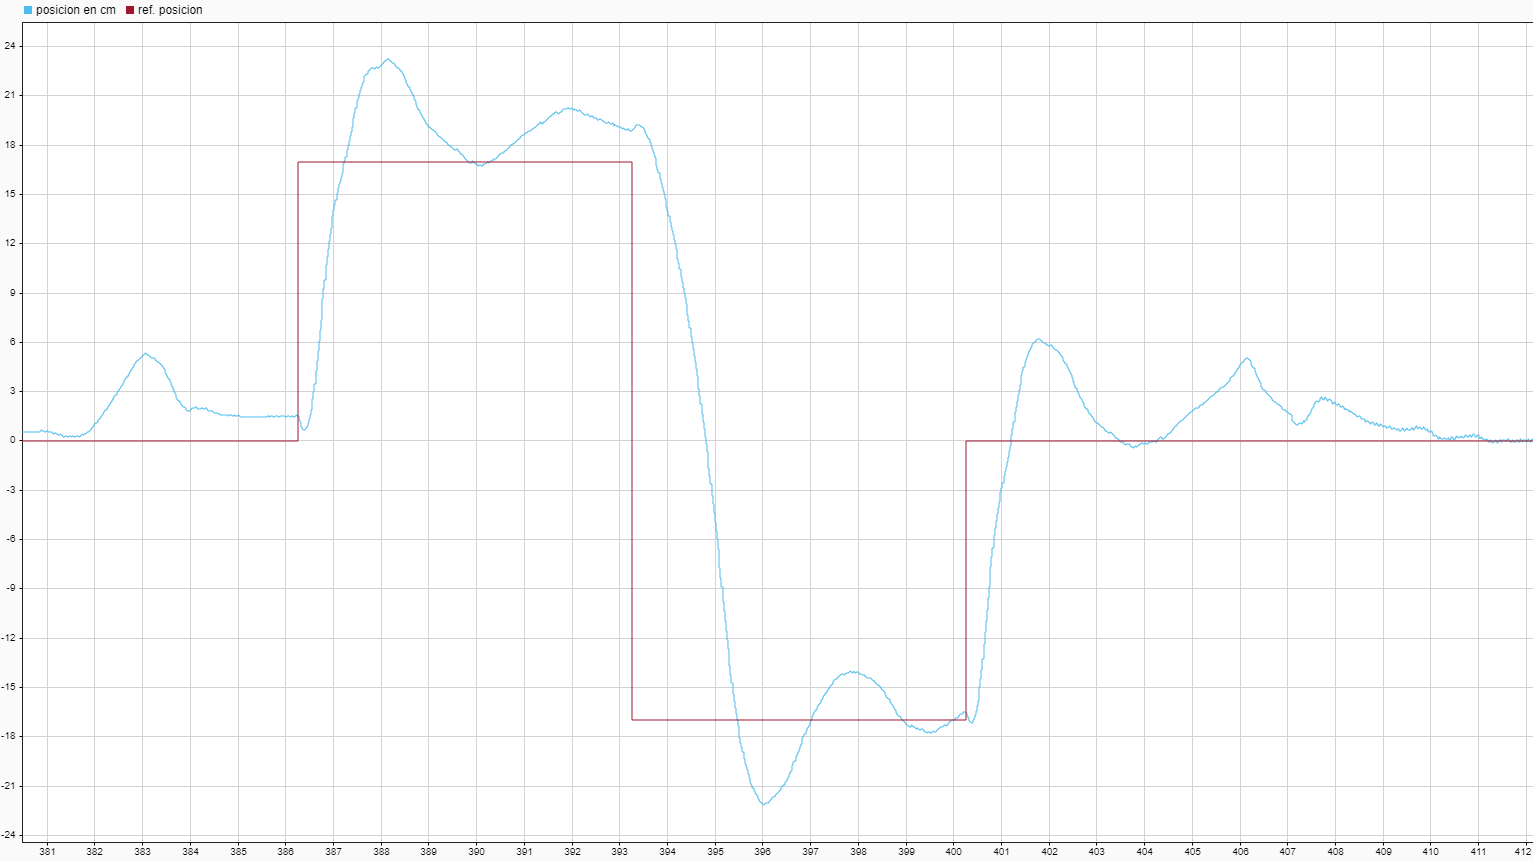
\includegraphics[width=0.6\textwidth]{Imagenes/Test Cambio de posicion/1-PID-pos.png}
    \caption{1 PID pos}
    \label{fig:1-PID-pos_0}
\end{figure}

\begin{figure}[H]
    \centering
    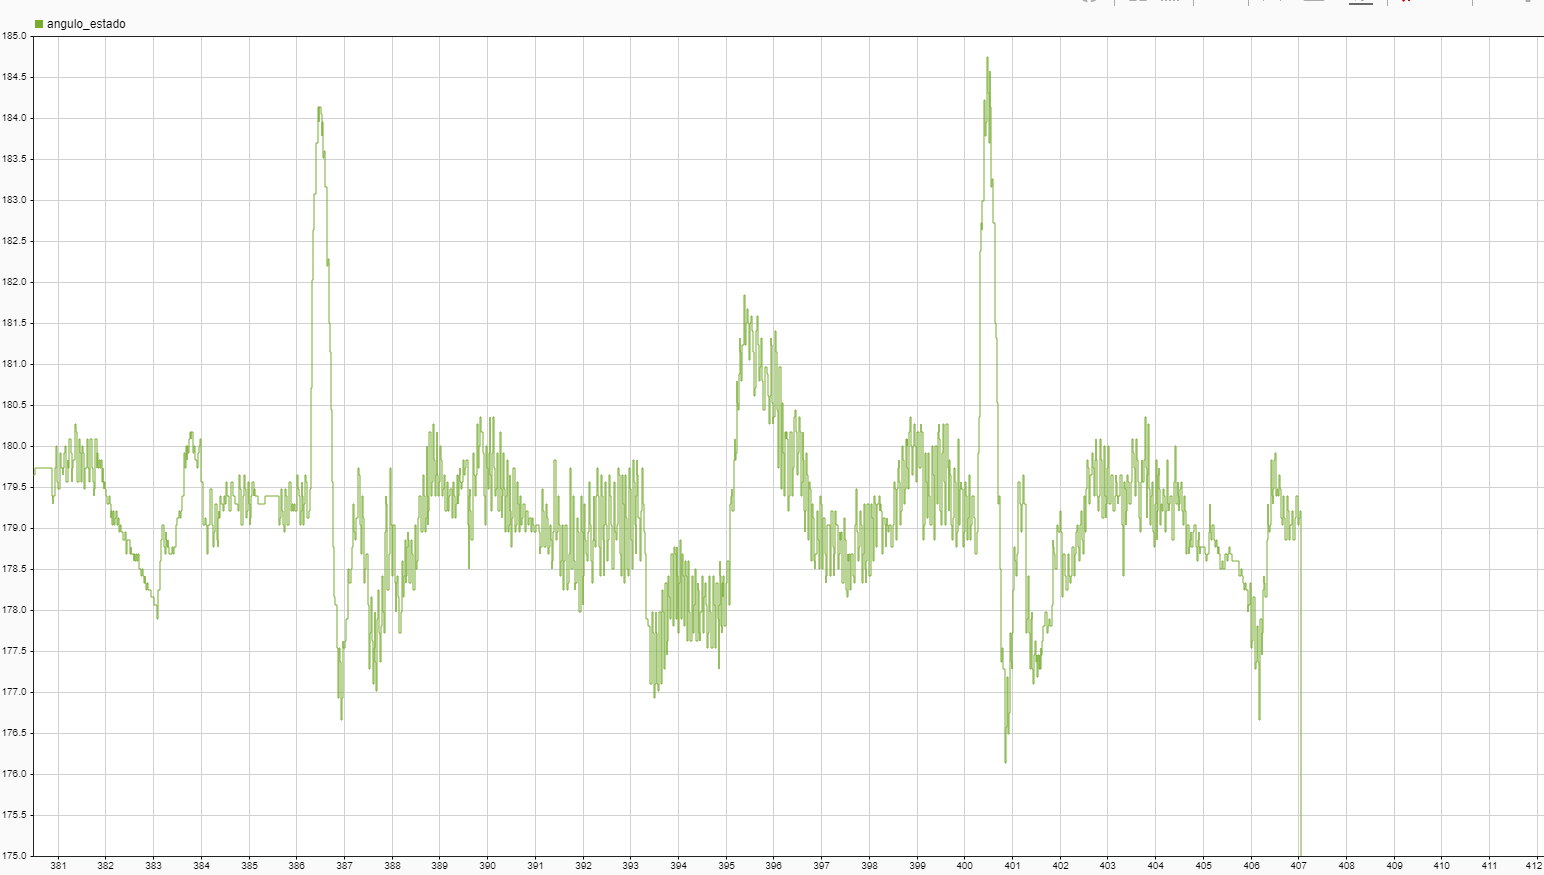
\includegraphics[width=0.6\textwidth]{Imagenes/Test Cambio de posicion/1-PID-angulo.png}
    \caption{1 PID angulo}
    \label{fig:1-PID-angulo_1}
\end{figure}

\begin{figure}[H]
    \centering
    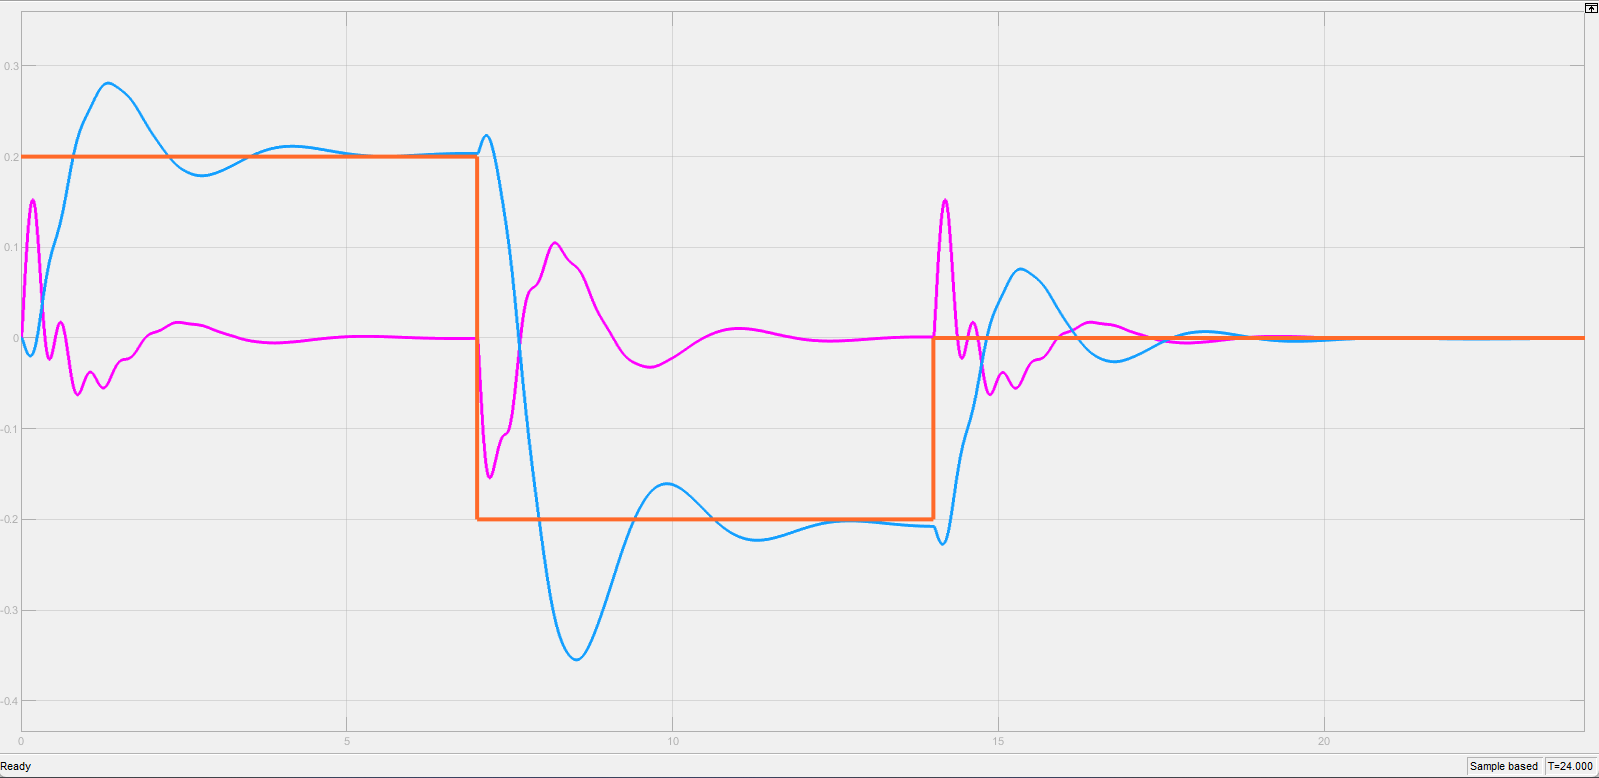
\includegraphics[width=0.6\textwidth]{Imagenes/Test Cambio de posicion/1-PID-sim.png}
    \caption{1 PID sim}
    \label{fig:1-PID-sim_2}
\end{figure}

\clearpage

\begin{figure}[H]
    \centering
    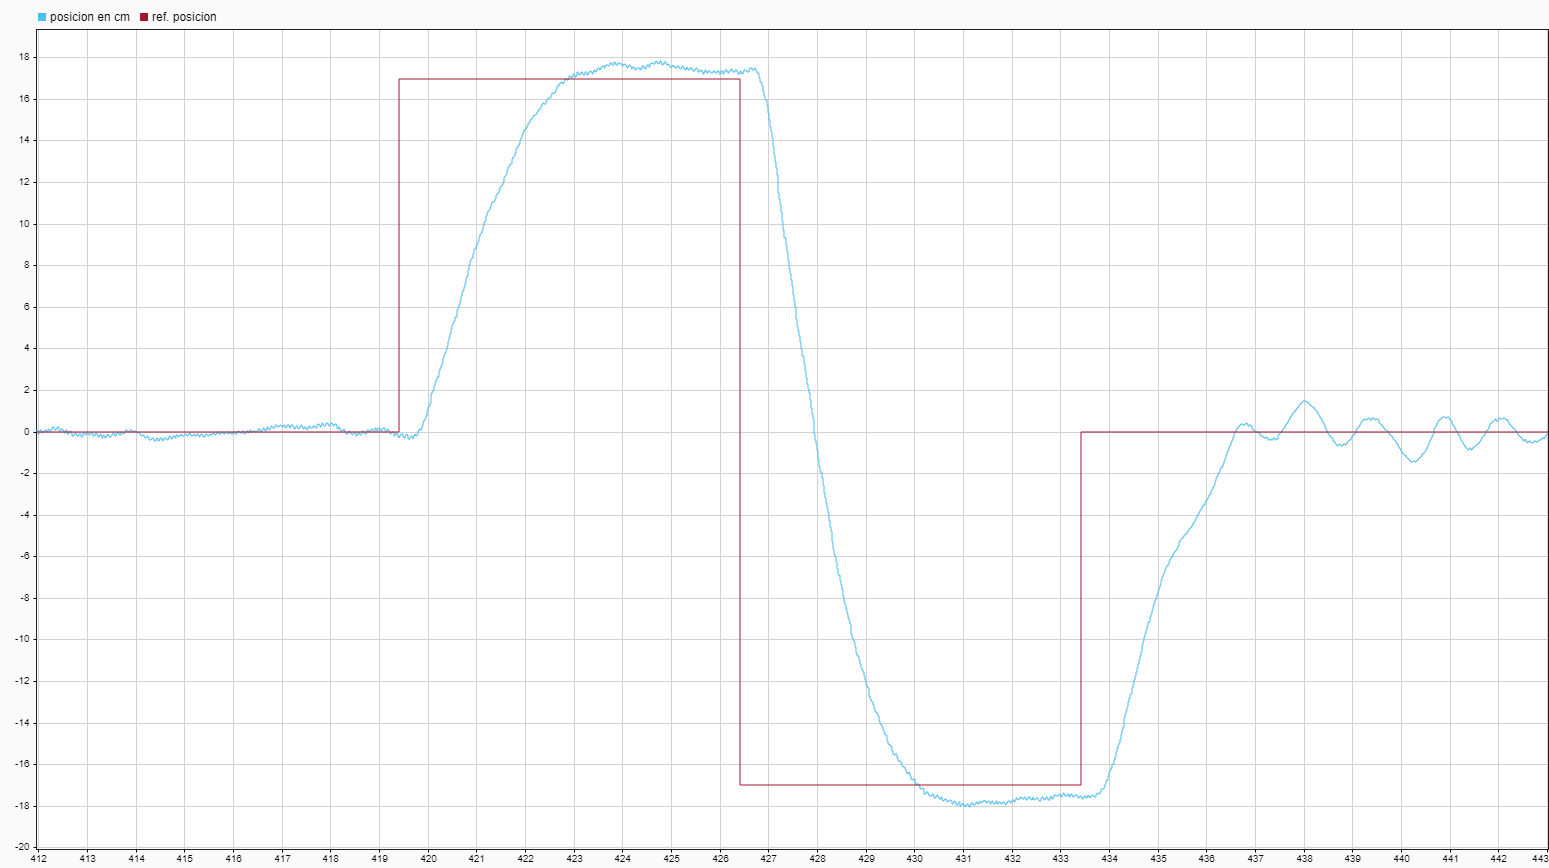
\includegraphics[width=0.6\textwidth]{Imagenes/Test Cambio de posicion/2-Identidad-pos.png}
    \caption{2 Identidad pos}
    \label{fig:2-Identidad-pos_3}
\end{figure}

\begin{figure}[H]
    \centering
    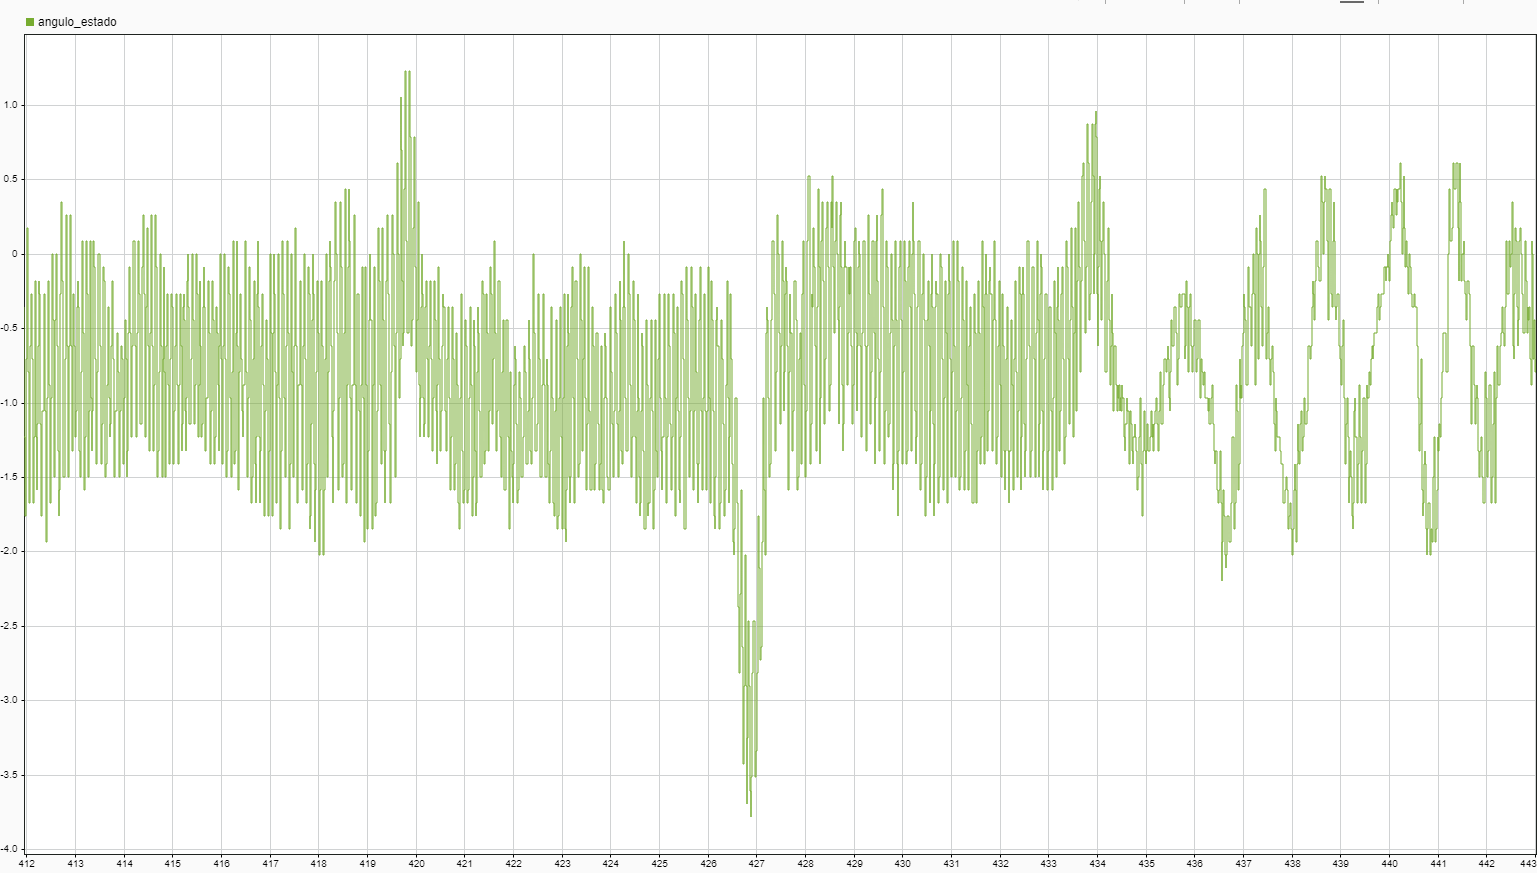
\includegraphics[width=0.6\textwidth]{Imagenes/Test Cambio de posicion/2-Identidad-angulo.png}
    \caption{2 Identidad angulo}
    \label{fig:2-Identidad-angulo_4}
\end{figure}

\begin{figure}[H]
    \centering
    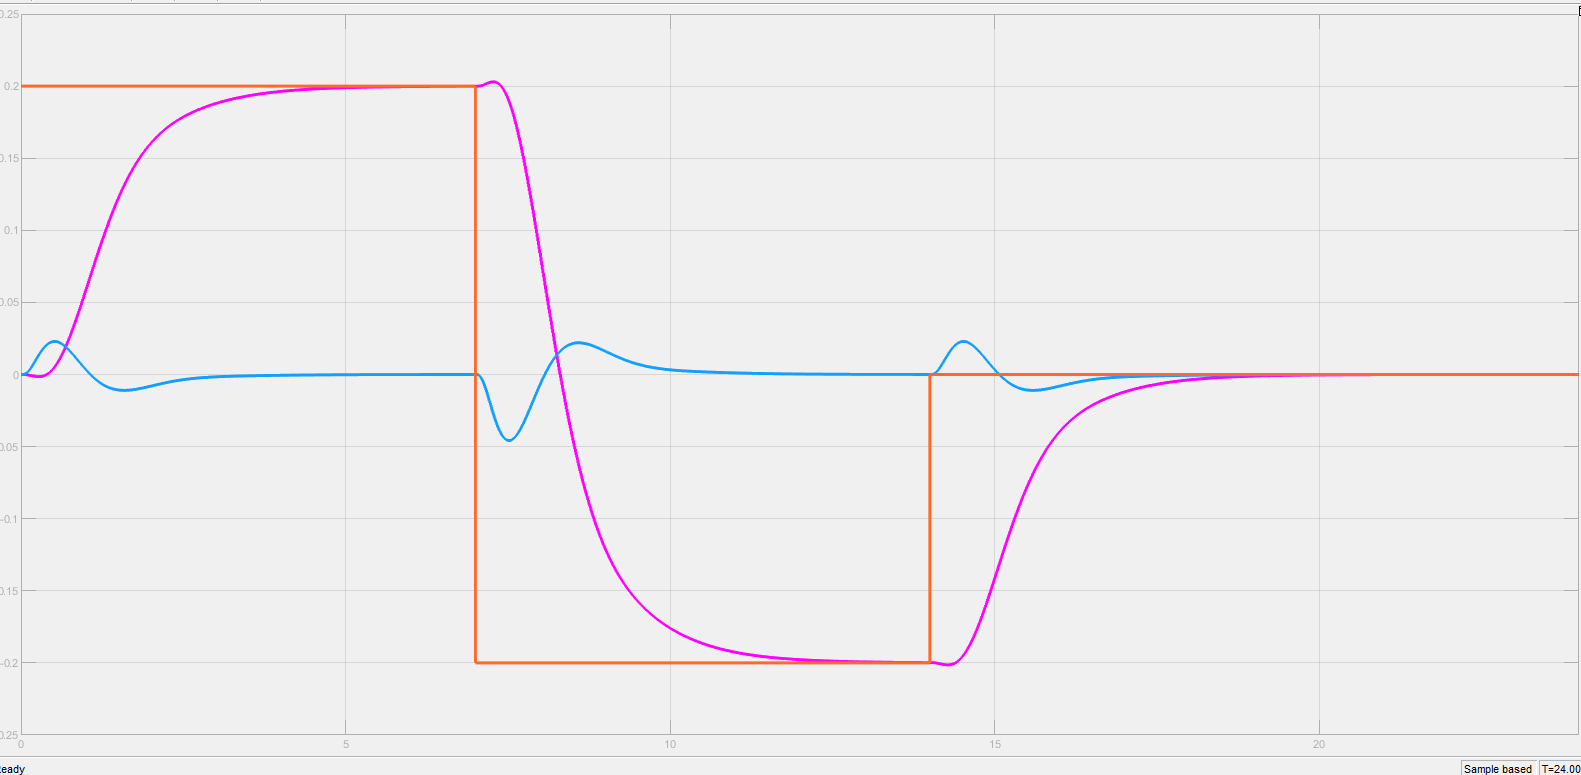
\includegraphics[width=0.6\textwidth]{Imagenes/Test Cambio de posicion/2-identidad-sim.png}
    \caption{2 Identidad sim}
    \label{fig:2-Identidad-sim-4}
\end{figure}

\clearpage

\begin{figure}[H]
    \centering
    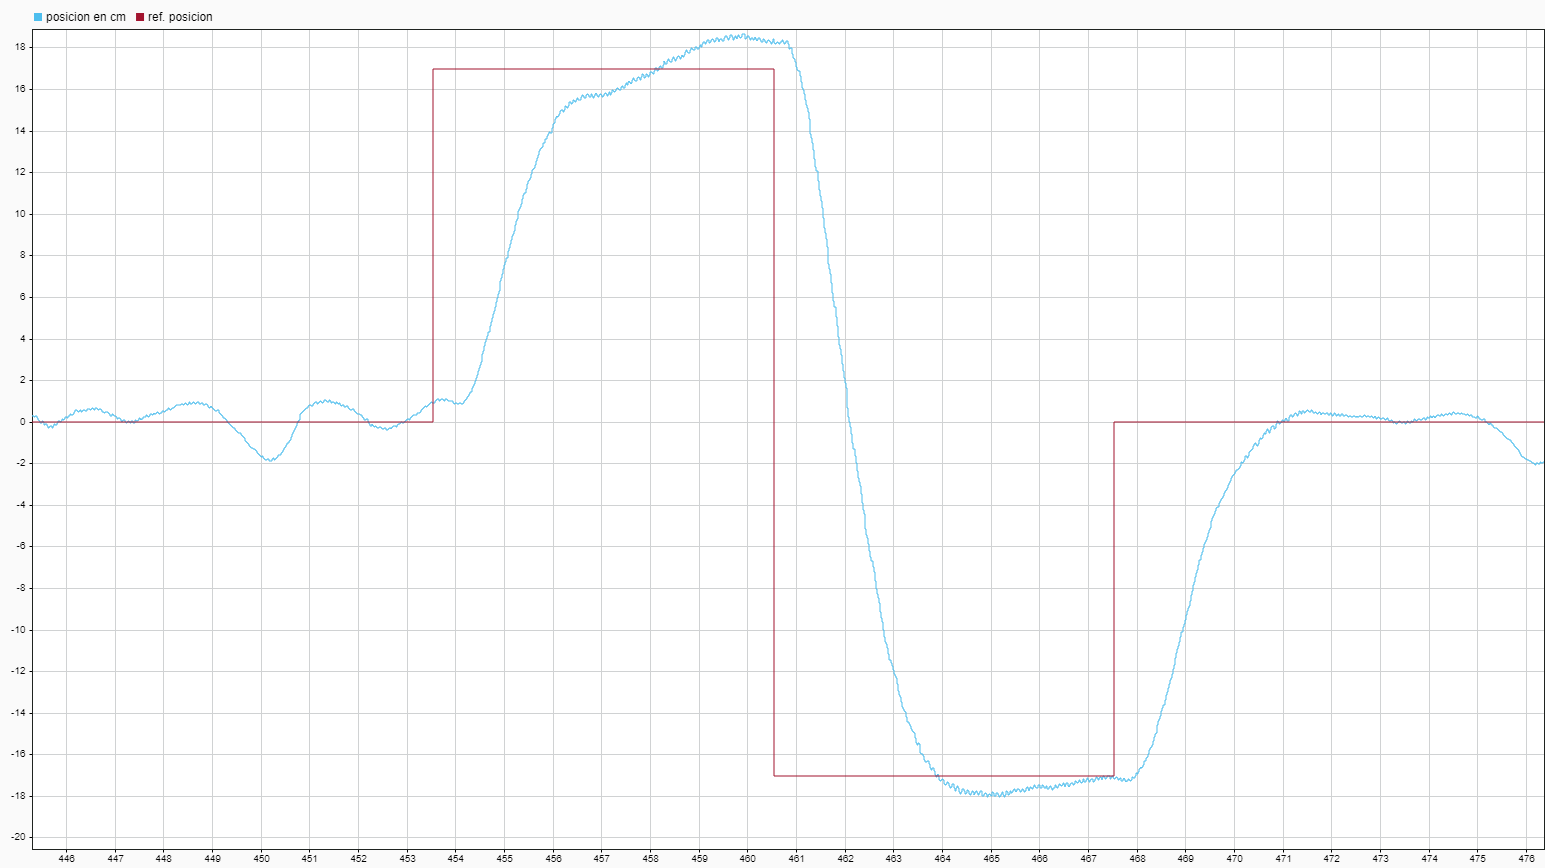
\includegraphics[width=0.6\textwidth]{Imagenes/Test Cambio de posicion/3-reducido-pos.png}
    \caption{3 reducido pos}
    \label{fig:3-reducido-pos_5}
\end{figure}


\begin{figure}[H]
    \centering
    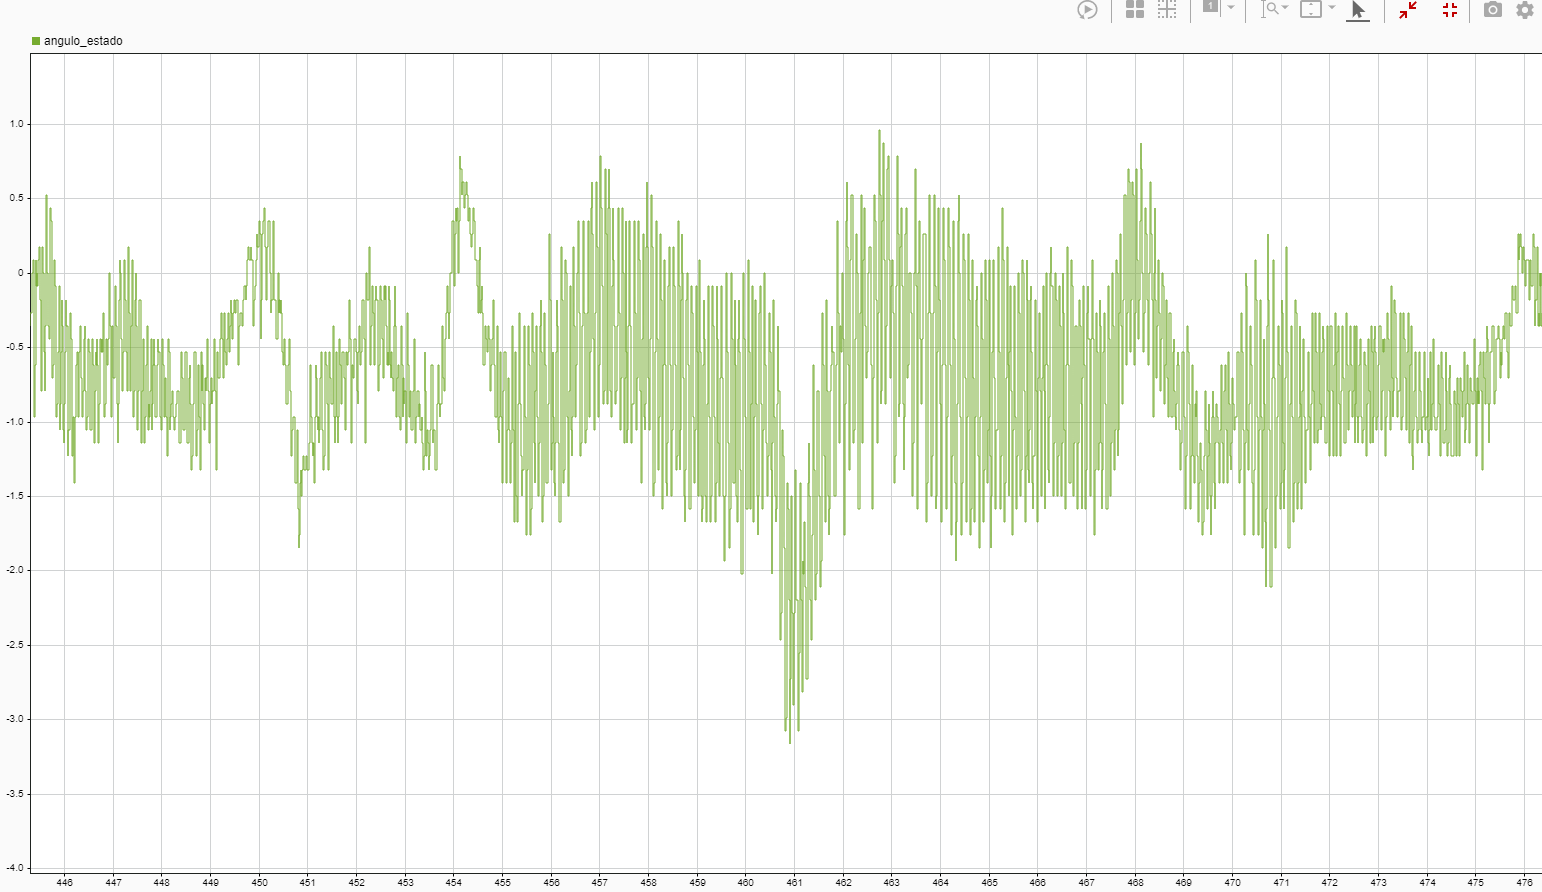
\includegraphics[width=0.6\textwidth]{Imagenes/Test Cambio de posicion/3-reducido-angulo.png}
    \caption{3 reducido angulo}
    \label{fig:3-reducido-angulo_6}
\end{figure}

\begin{figure}[H]
    \centering
    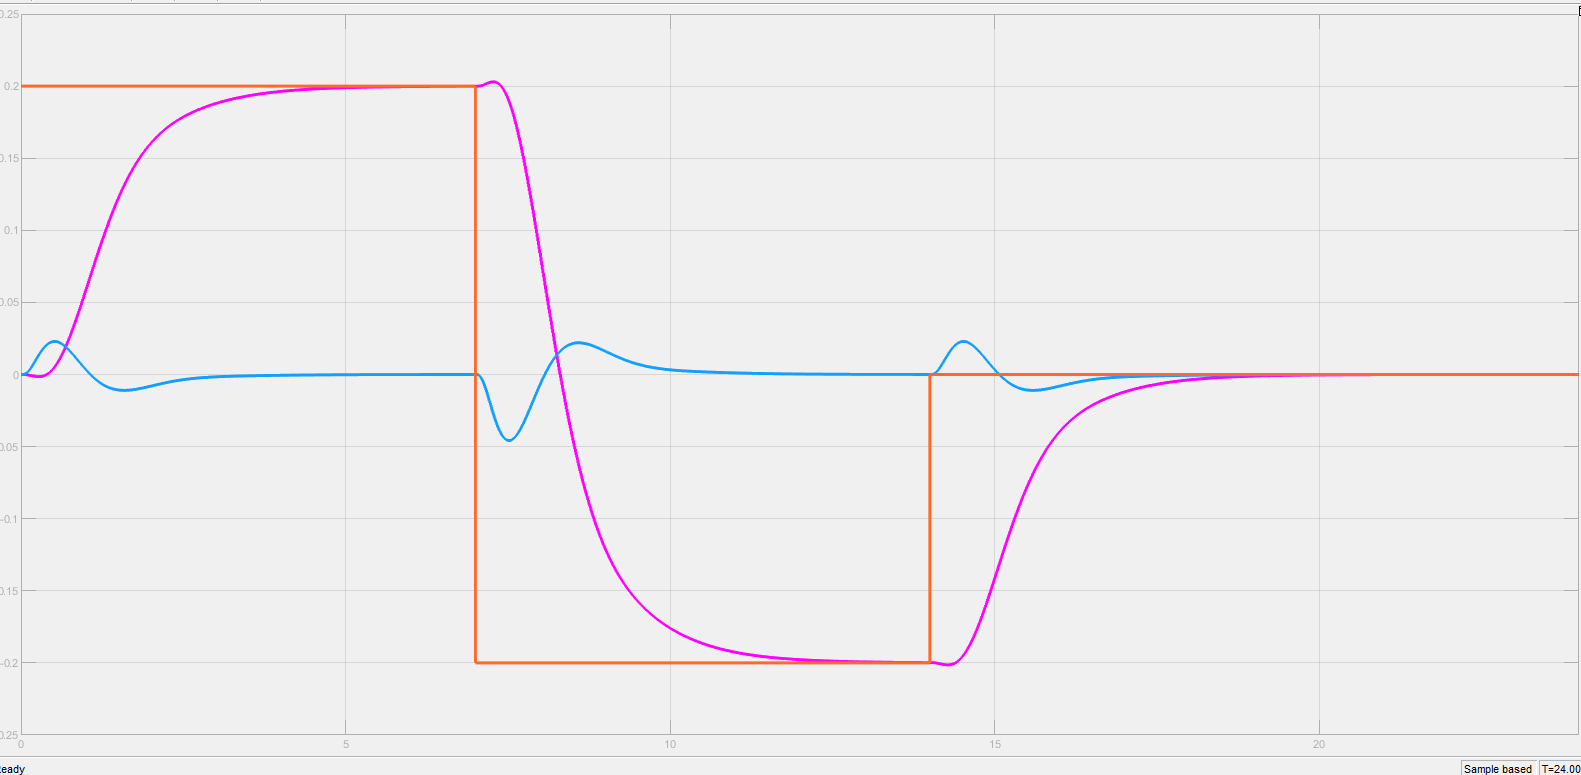
\includegraphics[width=0.6\textwidth]{Imagenes/Test Cambio de posicion/3-reducido-sim.png}
    \caption{3 reducido sim}
    \label{fig:3-reducido-sim_7}
\end{figure}

\clearpage

\begin{figure}[H]
    \centering
    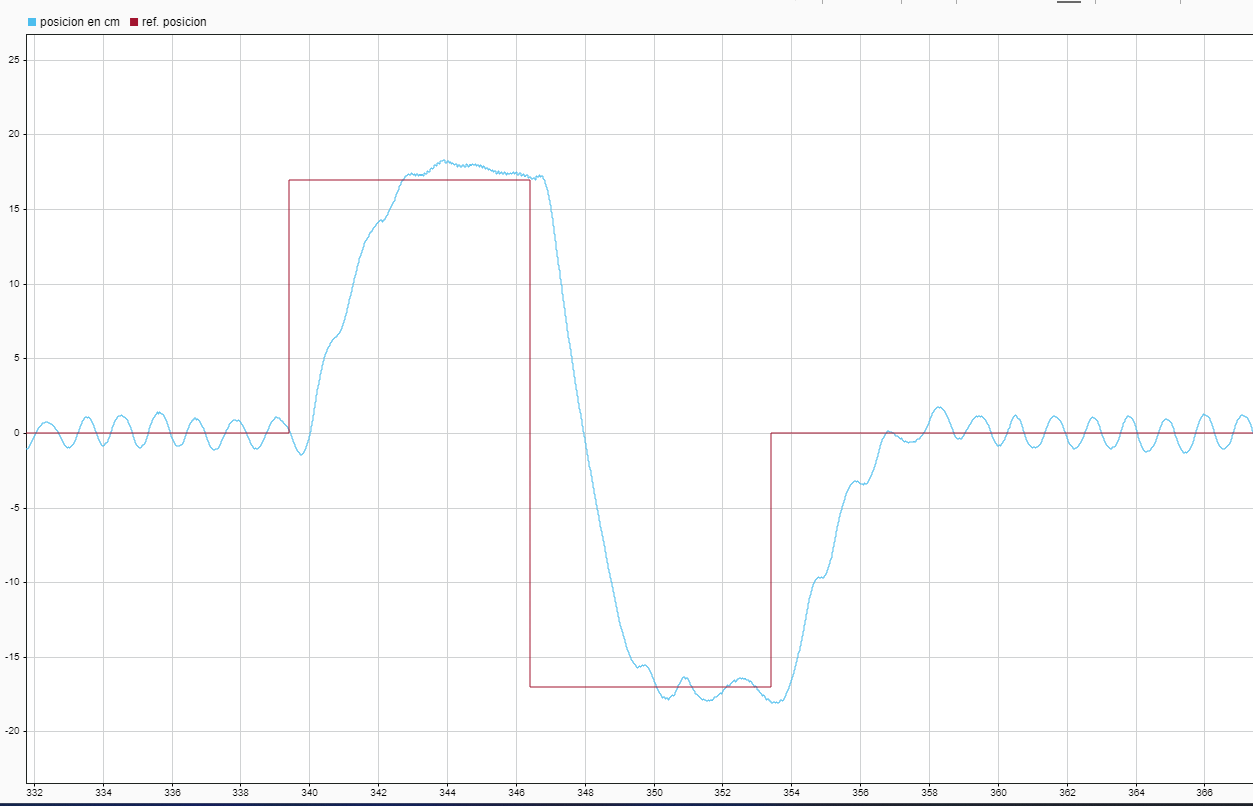
\includegraphics[width=0.6\textwidth]{Imagenes/Test Cambio de posicion/4-funcional_lineal-pos.png}
    \caption{4 funcional lineal pos}
    \label{fig:4-funcional_lineal-pos_8}
\end{figure}

\begin{figure}[H]
    \centering
    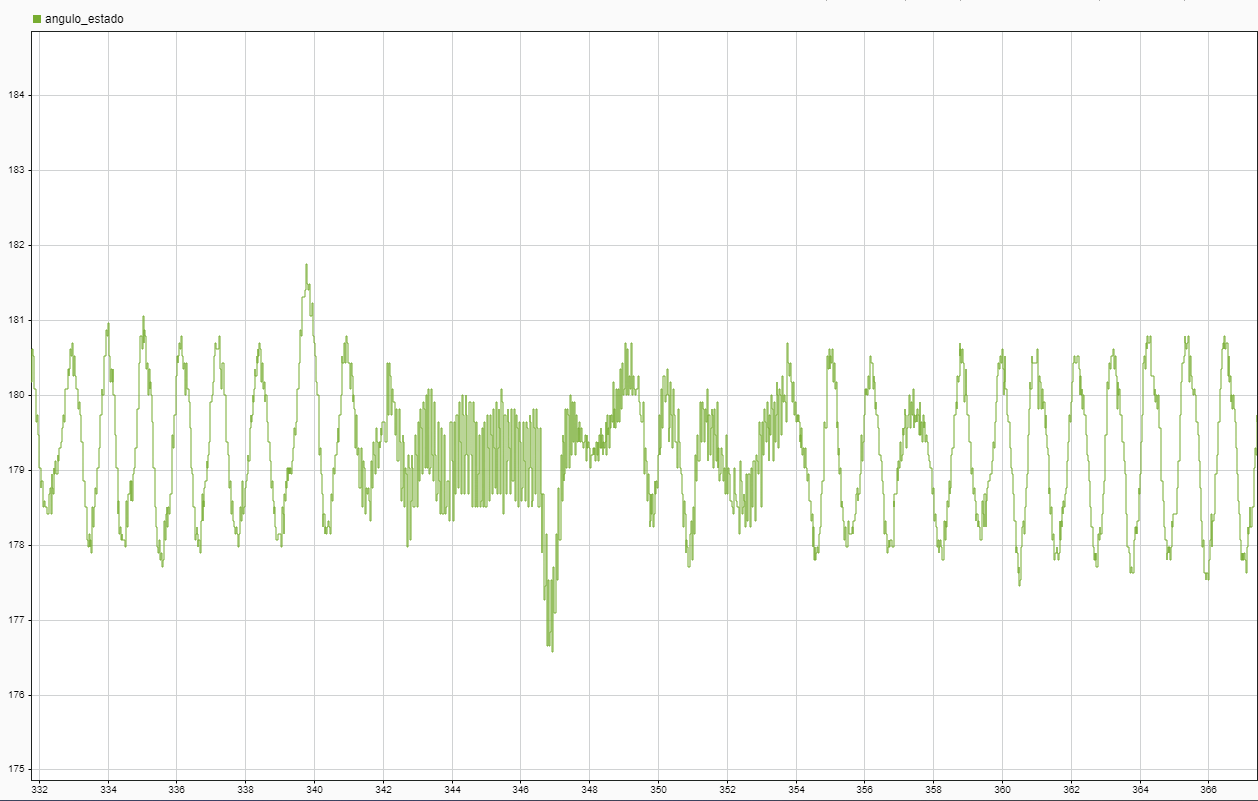
\includegraphics[width=0.6\textwidth]{Imagenes/Test Cambio de posicion/4-funcional-lineal-angulo.png}
    \caption{4 funcional lineal angulo}
    \label{fig:4-funcional-lineal-angulo_9}
\end{figure}

\begin{figure}[H]
    \centering
    \includegraphics[width=0.6\textwidth]{Imagenes/Test Cambio de posicion/4-funcional-lineal-sim.png}
    \caption{4 funcional lineal angulo}
    \label{fig:4-funcional-lineal-sim_9}
\end{figure}

\clearpage

\subsection{Test perturbación ángulo}

\begin{figure}[H]
    \centering
    
\includegraphics[width=0.6\textwidth]{Imagenes/Test Perturbacion angulo/1-PID-pos.png}
    \caption{1 PID pos}
    \label{fig:1-PID-pos_0}
\end{figure}

\begin{figure}[H]
    \centering
    
\includegraphics[width=0.6\textwidth]{Imagenes/Test Perturbacion angulo/1-PID-angulo.png}
    \caption{1 PID angulo}
    \label{fig:1-PID-angulo_1}
\end{figure}

\clearpage

\begin{figure}[H]
    \centering
    
\includegraphics[width=0.6\textwidth]{Imagenes/Test Perturbacion angulo/2-Identidad-pos.png}
    \caption{2 Identidad pos}
    \label{fig:2-Identidad-pos_3}
\end{figure}

\begin{figure}[H]
    \centering
    
\includegraphics[width=0.6\textwidth]{Imagenes/Test Perturbacion angulo/2-Identidad-angulo.png}
    \caption{2 Identidad angulo}
    \label{fig:2-Identidad-angulo_4}
\end{figure}

\clearpage

\begin{figure}[H]
    \centering
    
\includegraphics[width=0.6\textwidth]{Imagenes/Test Perturbacion angulo/3-reducido-pos.png}
    \caption{3 reducido pos}
    \label{fig:3-reducido-pos_5}
\end{figure}


\begin{figure}[H]
    \centering
    
\includegraphics[width=0.6\textwidth]{Imagenes/Test Perturbacion angulo/3-reducido-angulo.png}
    \caption{3 reducido angulo}
    \label{fig:3-reducido-angulo_6}
\end{figure}

\clearpage

\begin{figure}[H]
    \centering
    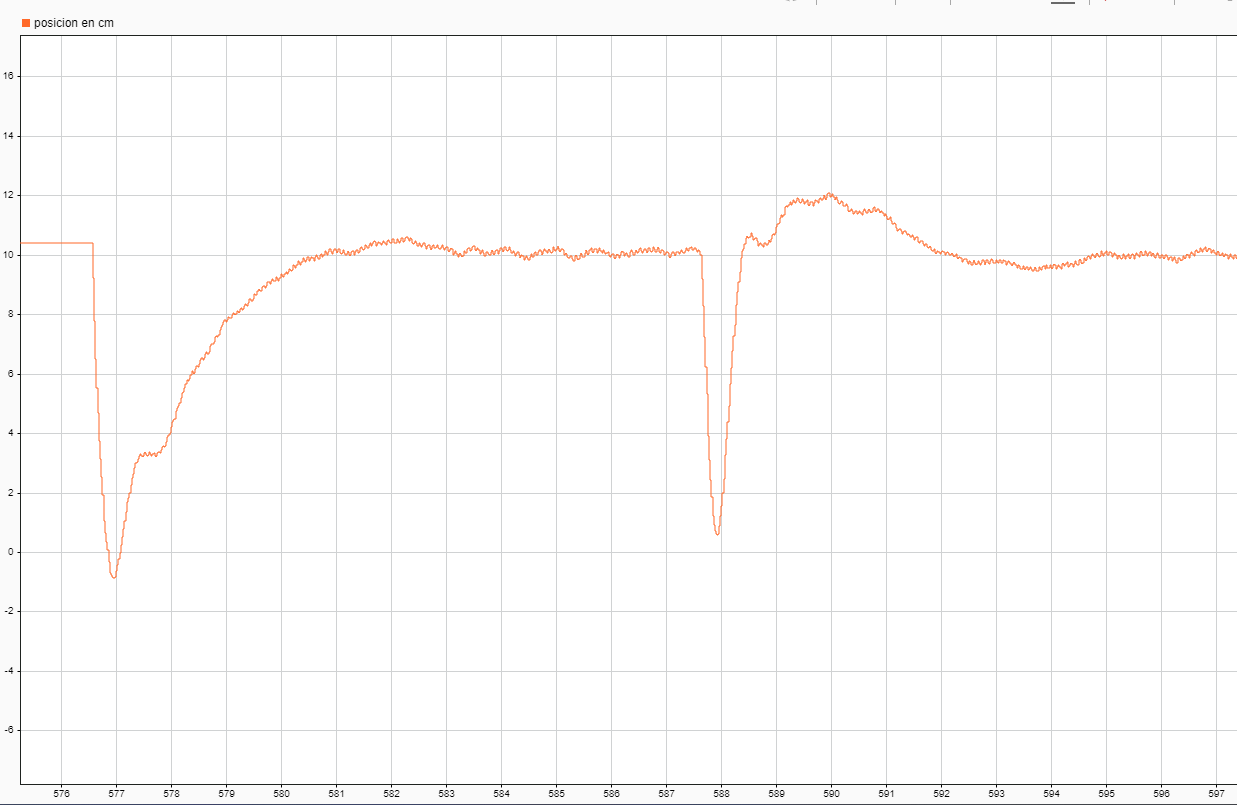
\includegraphics[width=0.6\textwidth]{Imagenes/Test Perturbacion angulo/4-funcional-pos.png}
    \caption{4 funcional pos}
    \label{fig:4-funcional-pos_8}
\end{figure}

\clearpage

\begin{figure}[H]
    \centering
    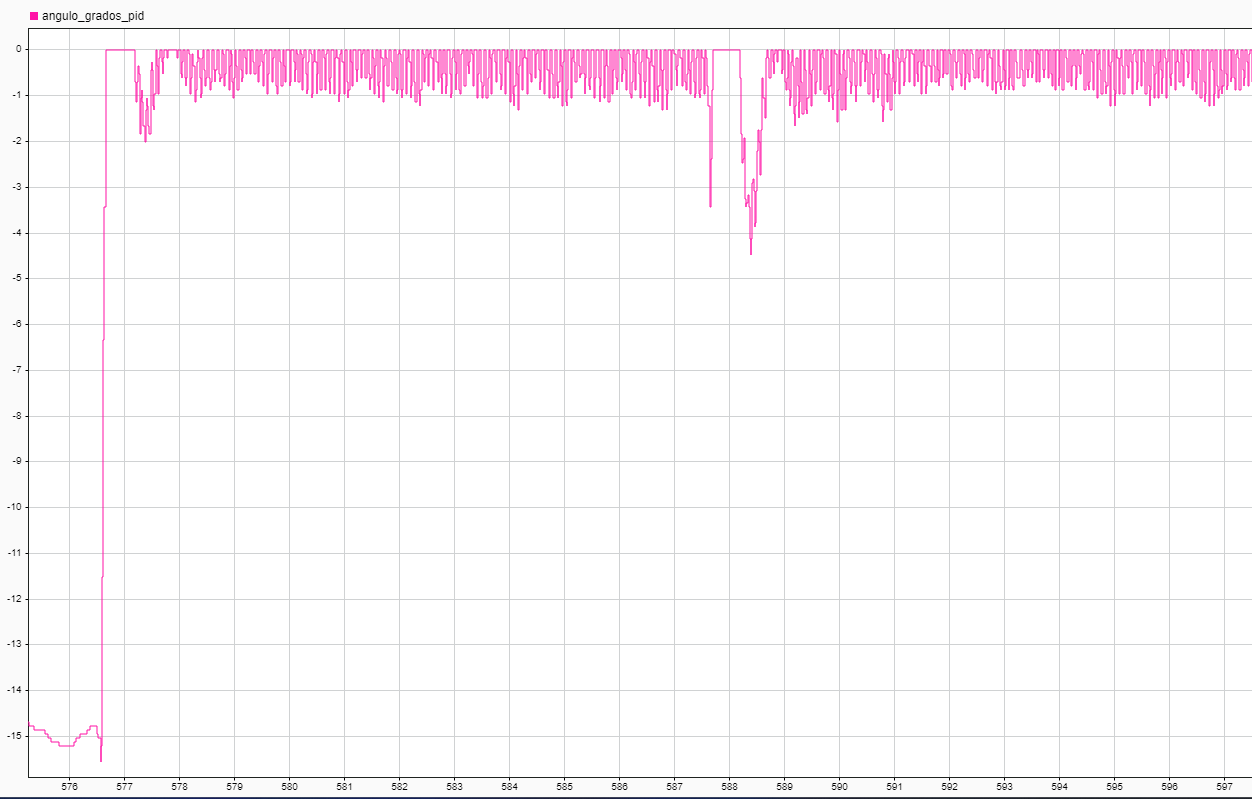
\includegraphics[width=0.6\textwidth]{Imagenes/Test Perturbacion angulo/4-funcional-angulo.png}
    \caption{4 funcional angulo}
    \label{fig:4-funcional-angulo_9}
\end{figure}


\end{document}